\documentclass{beamer}
\usepackage{caption}
\usepackage{subfig}


\begin{document}
\title{WASABI: an emotion model}   
\author{Yao Lu} 
\date{} 

\maketitle

\begin{frame}
\frametitle{Goal}
Build an emotion model
\newline \newline \newline
Why?
\begin{itemize}
\item better games
\item better robots
\item just for fun
\item publish a paper
\end{itemize}
\end{frame}

\begin{frame}
\frametitle{Here is a paper}
WASABI: Affect Simulation for Agents with
Believable Interactivity 
\newline \newline \newline
A demo is provided!
\newline \newline \newline
Let's test it!
\begin{itemize}
\item What's the model?
\item How to test the model?
\item Demo time!!!
\end{itemize}
\end{frame}


\begin{frame}
\frametitle{The Model}
Basic Assumptions:
\begin{itemize}
\item \textbf{emotions as responses to events}: \\ positive and negative events as inputs to the model.
\item \textbf{every emotion is a point in a 3D space}: Pleasure-Arousal-Dominance space.
\item \textbf{every emotion is determined by three hidden variables}: \\
valence, mood and boredom.
\item \textbf{events only affect valence}: \\
positive events = increase of valence.\\
negative events = decrease of valence.
\end{itemize}
\end{frame}

\begin{frame}
\frametitle{Every emotion is a point in a 3D space}

\textbf{Three axis}:\\
pleasure $\leftrightarrow$ displeasure \\
arousal $\leftrightarrow$ sleepiness \\
dominance $\leftrightarrow$ submissiveness

\end{frame}

\begin{frame}
\frametitle{Every emotion is determined by three hidden variables}
\textbf{valence}: intrinsic attractiveness (positive valence) or aversiveness (negative valence) of an event, object, or situation \\
\textbf{mood }\\
\textbf{boredom}
\newline
\newline
\textbf{pleasure} = $\frac{1}{2}$ (\textbf{valence}+ \textbf{mood}) \\
\textbf{arousal} = $|$\textbf{valence}$|$ + \textbf{boredom} \\
\textbf{dominance} = ?

\begin{figure}[h!]
\captionsetup[subfigure]{labelformat=empty}
\centering
\subfloat[valence]{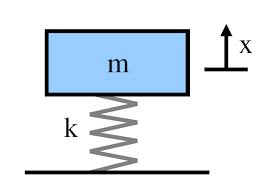
\includegraphics[scale=0.2]{mass_spring}} 
\subfloat[mood]{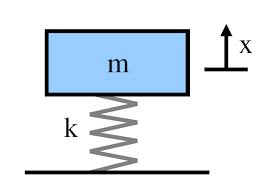
\includegraphics[scale=0.2]{mass_spring}} 
\subfloat[boredom]{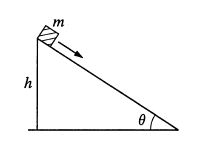
\includegraphics[scale=0.4]{mass_sliding}} 
\end{figure}
\end{frame}

\begin{frame}
\frametitle{The Model}
(valence, mood, boredom) $\rightarrow$ 
(pleasure, arousal, dominance) $\rightarrow$ \\
emotions
\end{frame}

\begin{frame}
\frametitle{Tests}
\end{frame}

\end{document}